% This is part of Un soupçon de mathématique sans être agressif pour autant
% Copyright (c) 2015
%   Laurent Claessens
% See the file fdl-1.3.txt for copying conditions.


\begin{rituel}
 Voici le diagramme semi-circulaire représentant la répartition de la population française par tranches d'âge en 2008 (INSEE).


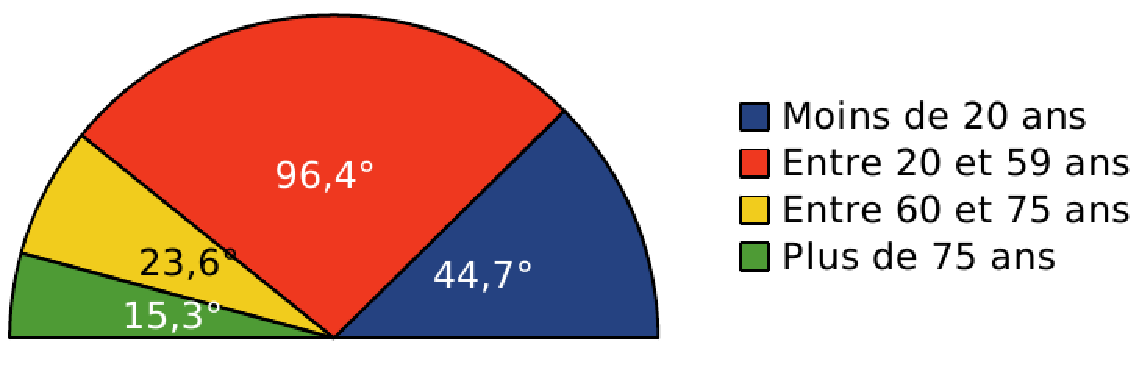
\includegraphics[width=0.8\linewidth]{diagsspop.pdf}


Sachant qu'en 2008 il y avait environ 63,7 millions d'habitants en France, construire le tableau des effectifs représentant ces catégories. 

\end{rituel}
